\documentclass[11pt,a4paper]{report}

% ============================================================================
% PACKAGES
% ============================================================================
\usepackage[utf8]{inputenc}
\usepackage[T1]{fontenc}
\usepackage[margin=1in]{geometry}
\usepackage{graphicx}
\usepackage{xcolor}
\usepackage{titlesec}
\usepackage{titletoc}
\usepackage{fancyhdr}
\usepackage{hyperref}
\usepackage{booktabs}
\usepackage{longtable}
\usepackage{array}
\usepackage{tabularx}
\usepackage{multirow}
\usepackage{enumitem}
\usepackage{tcolorbox}
\usepackage{tikz}
\usepackage{pgfplots}
\usepackage{pifont}
\usepackage{calc}
\usepackage{etoolbox}

\pgfplotsset{compat=1.18}
\usetikzlibrary{shapes.geometric, arrows.meta, positioning, calc, decorations.pathreplacing}

% ============================================================================
% COLOR DEFINITIONS
% ============================================================================
\definecolor{primaryblue}{RGB}{0, 82, 147}
\definecolor{secondaryblue}{RGB}{70, 130, 180}
\definecolor{accentorange}{RGB}{230, 126, 34}
\definecolor{accentgreen}{RGB}{39, 174, 96}
\definecolor{accentpurple}{RGB}{142, 68, 173}
\definecolor{lightgray}{RGB}{245, 245, 245}
\definecolor{darkgray}{RGB}{60, 60, 60}
\definecolor{trackA}{RGB}{41, 128, 185}
\definecolor{trackB}{RGB}{39, 174, 96}
\definecolor{trackC}{RGB}{142, 68, 173}
\definecolor{trackD}{RGB}{230, 126, 34}

% ============================================================================
% HYPERREF CONFIGURATION
% ============================================================================
\hypersetup{
    colorlinks=true,
    linkcolor=primaryblue,
    filecolor=primaryblue,
    urlcolor=secondaryblue,
    pdftitle={Comprehensive Systems Engineering and Software Architecture Curriculum},
    pdfauthor={Professional Development Program},
    pdfsubject={Systems Thinking, Software Architecture, and Engineering},
    bookmarksopen=true,
}

% ============================================================================
% TITLE FORMATTING
% ============================================================================
\titleformat{\chapter}[display]
    {\normalfont\huge\bfseries\color{primaryblue}}
    {\chaptertitlename\ \thechapter}{20pt}{\Huge}
\titleformat{\section}
    {\normalfont\Large\bfseries\color{primaryblue}}
    {\thesection}{1em}{}
\titleformat{\subsection}
    {\normalfont\large\bfseries\color{secondaryblue}}
    {\thesubsection}{1em}{}
\titleformat{\subsubsection}
    {\normalfont\normalsize\bfseries\color{darkgray}}
    {\thesubsubsection}{1em}{}

% ============================================================================
% HEADER AND FOOTER
% ============================================================================
\pagestyle{fancy}
\fancyhf{}
\fancyhead[L]{\small\leftmark}
\fancyhead[R]{\small Systems Engineering \& Software Architecture Curriculum}
\fancyfoot[C]{\thepage}
\renewcommand{\headrulewidth}{0.4pt}
\renewcommand{\footrulewidth}{0.4pt}

% ============================================================================
% CUSTOM BOXES
% ============================================================================
\newtcolorbox{learningobjectives}{
    colback=primaryblue!5,
    colframe=primaryblue,
    fonttitle=\bfseries,
    title={\ding{72} Learning Objectives},
    arc=3pt,
    boxrule=1pt,
    left=8pt,
    right=8pt,
    top=8pt,
    bottom=8pt
}

\newtcolorbox{keyinsight}{
    colback=accentorange!10,
    colframe=accentorange,
    fonttitle=\bfseries,
    title={\ding{72} Key Insight},
    arc=3pt,
    boxrule=1pt,
    left=8pt,
    right=8pt,
    top=6pt,
    bottom=6pt
}

\newtcolorbox{practicalexercise}{
    colback=accentgreen!10,
    colframe=accentgreen,
    fonttitle=\bfseries,
    title={\ding{72} Practical Exercise},
    arc=3pt,
    boxrule=1pt,
    left=8pt,
    right=8pt,
    top=6pt,
    bottom=6pt
}

\newtcolorbox{prerequisitebox}{
    colback=lightgray,
    colframe=darkgray,
    fonttitle=\bfseries,
    title={\ding{51} Prerequisites},
    arc=3pt,
    boxrule=1pt,
    left=8pt,
    right=8pt,
    top=6pt,
    bottom=6pt
}

\newtcolorbox{bookreference}{
    colback=accentpurple!5,
    colframe=accentpurple,
    fonttitle=\bfseries,
    arc=3pt,
    boxrule=1pt,
    left=8pt,
    right=8pt,
    top=6pt,
    bottom=6pt
}

\newtcolorbox{trackbox}[2][]{
    colback=#2!8,
    colframe=#2,
    fonttitle=\bfseries\large,
    title={#1},
    arc=4pt,
    boxrule=1.5pt,
    left=10pt,
    right=10pt,
    top=8pt,
    bottom=8pt
}

% ============================================================================
% CUSTOM COMMANDS
% ============================================================================
\newcommand{\duration}[1]{\textcolor{accentorange}{\ding{43} #1}}
\newcommand{\difficulty}[1]{\textcolor{secondaryblue}{\ding{115} #1}}
\newcommand{\bookicon}{\textcolor{accentpurple}{\ding{46}}}

% ============================================================================
% DOCUMENT BEGINS
% ============================================================================
\begin{document}

% Disable page anchors for title page to avoid duplicate identifiers
\hypersetup{pageanchor=false}

% ============================================================================
% TITLE PAGE
% ============================================================================
\begin{titlepage}
    \centering
    \vspace*{1cm}
    
    \begin{tikzpicture}[remember picture, overlay]
        \fill[primaryblue] (current page.north west) rectangle ([yshift=-4cm]current page.north east);
        \fill[secondaryblue] ([yshift=-4cm]current page.north west) rectangle ([yshift=-4.3cm]current page.north east);
    \end{tikzpicture}
    
    \vspace{2cm}
    
    {\Huge\bfseries\color{primaryblue} Comprehensive Curriculum}\\[0.5cm]
    {\Huge\bfseries\color{secondaryblue} in}\\[0.5cm]
    {\Huge\bfseries\color{primaryblue} Systems Engineering \&}\\[0.3cm]
    {\Huge\bfseries\color{primaryblue} Software Architecture}\\[1.5cm]
    
    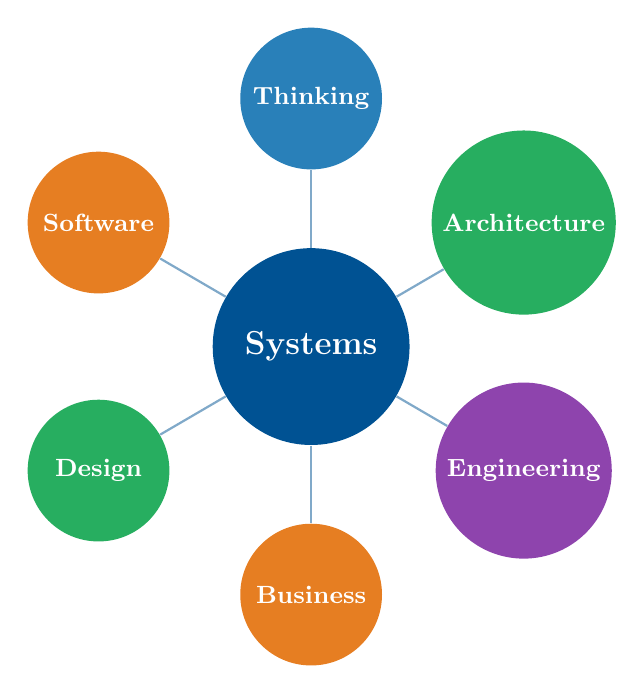
\begin{tikzpicture}[scale=0.9]
        % Central node
        \node[circle, fill=primaryblue, text=white, minimum size=2.5cm, font=\large\bfseries] (center) at (0,0) {Systems};
        
        % Surrounding nodes
        \node[circle, fill=trackA, text=white, minimum size=1.8cm, font=\small\bfseries] (thinking) at (0,3.5) {Thinking};
        \node[circle, fill=trackB, text=white, minimum size=1.8cm, font=\small\bfseries] (arch) at (3,1.75) {Architecture};
        \node[circle, fill=trackC, text=white, minimum size=1.8cm, font=\small\bfseries] (eng) at (3,-1.75) {Engineering};
        \node[circle, fill=trackD, text=white, minimum size=1.8cm, font=\small\bfseries] (business) at (0,-3.5) {Business};
        \node[circle, fill=accentgreen, text=white, minimum size=1.8cm, font=\small\bfseries] (design) at (-3,-1.75) {Design};
        \node[circle, fill=accentorange, text=white, minimum size=1.8cm, font=\small\bfseries] (software) at (-3,1.75) {Software};
        
        % Connecting lines
        \draw[thick, primaryblue!50] (center) -- (thinking);
        \draw[thick, primaryblue!50] (center) -- (arch);
        \draw[thick, primaryblue!50] (center) -- (eng);
        \draw[thick, primaryblue!50] (center) -- (business);
        \draw[thick, primaryblue!50] (center) -- (design);
        \draw[thick, primaryblue!50] (center) -- (software);
    \end{tikzpicture}
    
    \vspace{2cm}
    
    {\Large\color{darkgray} A Multi-Track Professional Development Program}\\[0.3cm]
    {\Large\color{darkgray} Integrating Theory, Practice, and Implementation}\\[2cm]
    
    {\large From Foundational Concepts to Advanced Applications}\\[0.5cm]
    {\large 16 Core Texts $\bullet$ 4 Learning Tracks $\bullet$ 52+ Week Program}\\[2cm]
    
    \begin{tikzpicture}[remember picture, overlay]
        \fill[primaryblue] (current page.south west) rectangle ([yshift=1cm]current page.south east);
    \end{tikzpicture}
    
\end{titlepage}

% ============================================================================
% TABLE OF CONTENTS
% ============================================================================
\hypersetup{pageanchor=true}
\pagenumbering{roman}
\tableofcontents
\thispagestyle{empty}
\clearpage

% Switch to Arabic numbering for main content
\pagenumbering{arabic}

% ============================================================================
% CHAPTER 1: INTRODUCTION AND OVERVIEW
% ============================================================================
\chapter{Introduction and Program Overview}

\section{Purpose and Scope}

This curriculum provides a structured, comprehensive pathway for developing expertise in systems engineering, software architecture, and business systems design. The program synthesizes insights from sixteen carefully selected texts spanning theoretical foundations, practical implementation strategies, and industry best practices.

The curriculum is designed for software engineers, technical leads, architects, and professionals seeking to develop a holistic understanding of how complex systems---both technical and organizational---are conceived, designed, built, and maintained.

\begin{learningobjectives}
Upon completion of this curriculum, participants will be able to:
\begin{itemize}[leftmargin=*]
    \item Apply systems thinking principles to analyze and solve complex problems at multiple scales
    \item Design and architect software systems that are reliable, scalable, and maintainable
    \item Understand and apply distributed systems principles in real-world applications
    \item Build and optimize business processes and organizational systems
    \item Apply object-oriented design principles effectively in software development
    \item Navigate the human and organizational aspects of software engineering projects
    \item Integrate theoretical knowledge with practical implementation skills
\end{itemize}
\end{learningobjectives}

\section{Program Structure}

The curriculum is organized into four interconnected learning tracks, each building upon foundational concepts while developing specialized expertise:

\begin{center}
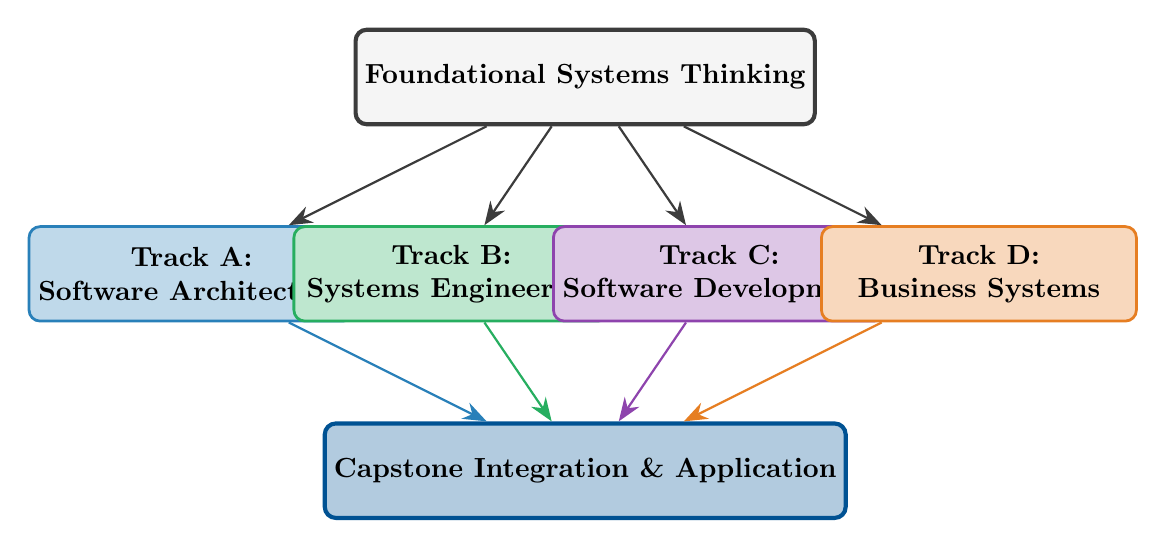
\begin{tikzpicture}[
    node distance=1.5cm,
    track/.style={rectangle, rounded corners, minimum width=4cm, minimum height=1.2cm, text centered, font=\bfseries, align=center},
    arrow/.style={-{Stealth[length=3mm]}, thick}
]
    % Foundation
    \node[track, fill=lightgray, draw=darkgray, line width=1.5pt] (foundation) at (0,0) {Foundational Systems Thinking};
    
    % Four tracks
    \node[track, fill=trackA!30, draw=trackA, line width=1pt] (trackA) at (-5,-2.5) {Track A:\\Software Architecture};
    \node[track, fill=trackB!30, draw=trackB, line width=1pt] (trackB) at (-1.7,-2.5) {Track B:\\Systems Engineering};
    \node[track, fill=trackC!30, draw=trackC, line width=1pt] (trackC) at (1.7,-2.5) {Track C:\\Software Development};
    \node[track, fill=trackD!30, draw=trackD, line width=1pt] (trackD) at (5,-2.5) {Track D:\\Business Systems};
    
    % Integration
    \node[track, fill=primaryblue!30, draw=primaryblue, line width=1.5pt] (integration) at (0,-5) {Capstone Integration \& Application};
    
    % Arrows from foundation
    \draw[arrow, darkgray] (foundation) -- (trackA);
    \draw[arrow, darkgray] (foundation) -- (trackB);
    \draw[arrow, darkgray] (foundation) -- (trackC);
    \draw[arrow, darkgray] (foundation) -- (trackD);
    
    % Arrows to integration
    \draw[arrow, trackA] (trackA) -- (integration);
    \draw[arrow, trackB] (trackB) -- (integration);
    \draw[arrow, trackC] (trackC) -- (integration);
    \draw[arrow, trackD] (trackD) -- (integration);
    
\end{tikzpicture}
\end{center}

\section{Core Reading List Overview}

The curriculum integrates the following sixteen core texts, organized by primary focus area:

\subsection{Foundational Systems Thinking}

\begin{longtable}{>{\raggedright\arraybackslash}p{5.5cm} >{\raggedright\arraybackslash}p{4cm} >{\raggedright\arraybackslash}p{4.5cm}}
\toprule
\textbf{Title} & \textbf{Author(s)} & \textbf{Primary Focus} \\
\midrule
\endhead
Thinking in Systems: A Primer & Donella H. Meadows & Systems dynamics and mental models \\
An Introduction to General Systems Thinking & Gerald M. Weinberg & General systems theory \\
\bottomrule
\end{longtable}

\subsection{Computer Systems and Software Architecture}

\begin{longtable}{>{\raggedright\arraybackslash}p{5.5cm} >{\raggedright\arraybackslash}p{4cm} >{\raggedright\arraybackslash}p{4.5cm}}
\toprule
\textbf{Title} & \textbf{Author(s)} & \textbf{Primary Focus} \\
\midrule
\endhead
Designing Data-Intensive Applications & Martin Kleppmann & Distributed data systems \\
Distributed Systems: Principles and Paradigms & Tanenbaum \& van Steen & Distributed computing theory \\
Fundamentals of Software Architecture & Richards \& Ford & Architecture styles and patterns \\
Operating System Concepts & Silberschatz, Galvin, \& Gagne & OS internals and design \\
\bottomrule
\end{longtable}

\subsection{Software Engineering Practice}

\begin{longtable}{>{\raggedright\arraybackslash}p{5.5cm} >{\raggedright\arraybackslash}p{4cm} >{\raggedright\arraybackslash}p{4.5cm}}
\toprule
\textbf{Title} & \textbf{Author(s)} & \textbf{Primary Focus} \\
\midrule
\endhead
Practical Object-Oriented Design & Sandi Metz & OO design principles \\
The Mythical Man-Month & Frederick Brooks Jr. & Project management \\
Modern Software Engineering & David Farley & Contemporary practices \\
\bottomrule
\end{longtable}

\subsection{Systems Engineering}

\begin{longtable}{>{\raggedright\arraybackslash}p{5.5cm} >{\raggedright\arraybackslash}p{4cm} >{\raggedright\arraybackslash}p{4.5cm}}
\toprule
\textbf{Title} & \textbf{Author(s)} & \textbf{Primary Focus} \\
\midrule
\endhead
Systems Engineering Principles and Practice & Alexander Kossiakoff & SE methodology \\
The Art of Systems Engineering & Marco Chicherio & Practical SE application \\
\bottomrule
\end{longtable}

\subsection{Business Systems and Process Design}

\begin{longtable}{>{\raggedright\arraybackslash}p{5.5cm} >{\raggedright\arraybackslash}p{4cm} >{\raggedright\arraybackslash}p{4.5cm}}
\toprule
\textbf{Title} & \textbf{Author(s)} & \textbf{Primary Focus} \\
\midrule
\endhead
The E-Myth Revisited & Michael Gerber & Business systematization \\
Work the System & Sam Carpenter & Process documentation \\
Traction & Gino Wickman & Organizational structure \\
Scaling Up & Verne Harnish & Growth systems \\
Service Design Doing & Various & Process design methodology \\
\bottomrule
\end{longtable}

\section{Time Commitment and Pacing}

\begin{center}
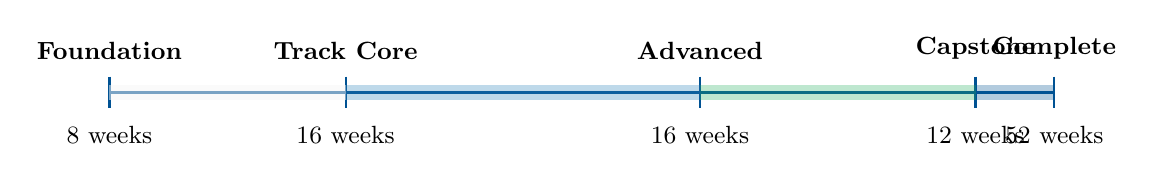
\begin{tikzpicture}
    \draw[thick, primaryblue] (0,0) -- (12,0);
    
    % Phase markers
    \foreach \x/\label/\weeks in {0/Foundation/8, 3/Track Core/16, 7.5/Advanced/16, 11/Capstone/12} {
        \draw[thick, primaryblue] (\x,0.2) -- (\x,-0.2);
        \node[above, font=\small\bfseries] at (\x,0.3) {\label};
        \node[below, font=\small] at (\x,-0.3) {\weeks{} weeks};
    }
    
    % End marker
    \draw[thick, primaryblue] (12,0.2) -- (12,-0.2);
    \node[above, font=\small\bfseries] at (12,0.3) {Complete};
    \node[below, font=\small] at (12,-0.3) {52 weeks};
    
    % Colored segments
    \fill[lightgray, opacity=0.5] (0,-0.1) rectangle (3,0.1);
    \fill[trackA, opacity=0.3] (3,-0.1) rectangle (7.5,0.1);
    \fill[accentgreen, opacity=0.3] (7.5,-0.1) rectangle (11,0.1);
    \fill[primaryblue, opacity=0.3] (11,-0.1) rectangle (12,0.1);
\end{tikzpicture}
\end{center}

The program is designed for approximately 52 weeks of study, assuming 10--15 hours of weekly commitment. This includes reading time, practical exercises, reflection activities, and project work. The pacing can be adjusted based on prior experience and available time.

% ============================================================================
% CHAPTER 2: FOUNDATIONAL PHASE
% ============================================================================
\chapter{Phase 1: Foundational Systems Thinking}

\duration{8 weeks} \hfill \difficulty{Beginner to Intermediate}

\vspace{0.5cm}

This foundational phase establishes the theoretical framework that underpins all subsequent learning. Systems thinking provides the mental models necessary for understanding complex technical and organizational systems, making it essential preparation for the specialized tracks.

\begin{learningobjectives}
\begin{itemize}[leftmargin=*]
    \item Understand the fundamental principles of systems dynamics
    \item Recognize feedback loops, leverage points, and emergent behavior
    \item Apply systems thinking to analyze real-world problems
    \item Develop vocabulary and frameworks for discussing complex systems
    \item Understand how systems can degrade and how to design for resilience
\end{itemize}
\end{learningobjectives}

\section{Module 1.1: Thinking in Systems}

\duration{4 weeks} \hfill \bookicon{} \textit{Thinking in Systems: A Primer} by Donella H. Meadows

\begin{bookreference}
\textbf{About This Book:} This concise guide is considered crucial for understanding problem-solving at scales ranging from personal to global. Meadows argues that many large-scale problems are fundamentally system failures, and this book develops the core skills needed to navigate an increasingly complex world for effective problem solving and decision making.
\end{bookreference}

\subsection{Week 1--2: Core Concepts}

\subsubsection{Reading Focus}
\begin{itemize}[leftmargin=*]
    \item Parts I and II: System structure and basic dynamics
    \item Focus on understanding stocks, flows, and feedback loops
    \item Study the iceberg model: events, patterns, structures, mental models
\end{itemize}

\subsubsection{Key Concepts to Master}

\textbf{Stocks and Flows:} Understanding accumulation and rates of change as the foundation of dynamic behavior. Stocks represent the state of a system at any point in time, while flows represent the rates of change that affect stocks.

\textbf{Feedback Loops:} Distinguishing between reinforcing (positive) and balancing (negative) feedback loops. Reinforcing loops amplify change, while balancing loops resist it and seek equilibrium.

\textbf{Delays:} Recognizing how time delays between cause and effect create oscillation, overshoot, and counterintuitive system behavior.

\begin{practicalexercise}
\textbf{Exercise 1.1: System Mapping}

Select a system you interact with daily (e.g., your morning routine, a software deployment pipeline, or your team's workflow). Create a causal loop diagram that identifies:
\begin{enumerate}[leftmargin=*]
    \item At least three stocks (quantities that accumulate)
    \item The flows that affect each stock
    \item Two reinforcing feedback loops
    \item Two balancing feedback loops
    \item Any significant delays in the system
\end{enumerate}
Document how these elements interact and predict what would happen if you intervened at different points.
\end{practicalexercise}

\subsection{Week 3--4: Leverage Points and System Archetypes}

\subsubsection{Reading Focus}
\begin{itemize}[leftmargin=*]
    \item Parts III and IV: System dynamics and places to intervene
    \item Meadows' famous ``Leverage Points'' framework
    \item Common system archetypes and their patterns
\end{itemize}

\subsubsection{Leverage Points Hierarchy}

Meadows identifies twelve leverage points, ranked from least to most effective:

\begin{enumerate}[leftmargin=*, start=12]
    \setcounter{enumi}{11}
    \item[12.] Constants, parameters, numbers
    \item[11.] Buffer sizes and stabilizing stocks
    \item[10.] Structure of material stocks and flows
    \item[9.] Delays in feedback loops
    \item[8.] Strength of negative feedback loops
    \item[7.] Gain of positive feedback loops
    \item[6.] Information flows
    \item[5.] Rules of the system
    \item[4.] Power to add, change, or evolve system structure
    \item[3.] Goals of the system
    \item[2.] Mindset or paradigm from which the system arises
    \item[1.] Transcending paradigms
\end{enumerate}

\begin{keyinsight}
The most powerful leverage points are often the least intuitive. While we naturally focus on adjustable parameters (like budgets or deadlines), the most effective interventions often involve changing information flows, rules, or the underlying mental models that shape the system.
\end{keyinsight}

\begin{practicalexercise}
\textbf{Exercise 1.2: Leverage Point Analysis}

Revisit the system you mapped in Exercise 1.1. For each of Meadows' twelve leverage points:
\begin{enumerate}[leftmargin=*]
    \item Identify where that leverage point exists in your system
    \item Assess the current state of that leverage point
    \item Propose a specific intervention at that point
    \item Predict the likely short-term and long-term effects
\end{enumerate}
Create a prioritized list of interventions based on expected impact versus implementation difficulty.
\end{practicalexercise}

\section{Module 1.2: General Systems Thinking}

\duration{4 weeks} \hfill \bookicon{} \textit{An Introduction to General Systems Thinking} by Gerald M. Weinberg

\begin{bookreference}
\textbf{About This Book:} This foundational text explores general systems thinking concepts with wit and practicality. Weinberg offers profound insights for navigating complex organizational challenges, making it essential reading alongside Meadows' work as a key text in the field.
\end{bookreference}

\subsection{Week 5--6: Foundations of Observation}

\subsubsection{Reading Focus}
\begin{itemize}[leftmargin=*]
    \item The problem of observation and description
    \item Science and its limitations in understanding complex systems
    \item The observer's role in defining and bounding systems
\end{itemize}

\subsubsection{Key Concepts to Master}

\textbf{The Law of Medium Numbers:} Systems in the ``medium number'' range (too complex for simple analysis, too small for statistical methods) require systems thinking approaches.

\textbf{The Complementarity Principle:} No single view of a complex system is complete; multiple perspectives are necessary for understanding.

\textbf{The Generalized Thermodynamic Interpretation:} Understanding how systems tend toward disorder and the energy required to maintain organization.

\subsection{Week 7--8: Decomposition and Behavior}

\subsubsection{Reading Focus}
\begin{itemize}[leftmargin=*]
    \item Interpreting behavior and change
    \item System decomposition strategies
    \item The relationship between structure and behavior
\end{itemize}

\begin{practicalexercise}
\textbf{Exercise 1.3: Multi-Perspective System Analysis}

Choose a complex technical system (e.g., a microservices architecture, a CI/CD pipeline, or an e-commerce platform). Analyze it from at least four different perspectives:
\begin{enumerate}[leftmargin=*]
    \item The end user's perspective
    \item The developer's perspective
    \item The operations team's perspective
    \item The business stakeholder's perspective
\end{enumerate}
For each perspective, document:
\begin{itemize}[leftmargin=*]
    \item What elements of the system are visible?
    \item What elements are hidden or abstracted away?
    \item What behaviors are most important?
    \item What constitutes ``success'' or ``failure''?
\end{itemize}
Synthesize these views to identify tensions and trade-offs inherent in the system design.
\end{practicalexercise}

\section{Phase 1 Assessment Checkpoint}

Before proceeding to the specialized tracks, participants should be able to:

\begin{itemize}[leftmargin=*]
    \item[\ding{51}] Draw and interpret causal loop diagrams for complex systems
    \item[\ding{51}] Identify feedback loops and predict their effects
    \item[\ding{51}] Apply the leverage points framework to real problems
    \item[\ding{51}] Recognize common system archetypes in technical and organizational contexts
    \item[\ding{51}] Articulate the observer's role in defining system boundaries
    \item[\ding{51}] Integrate multiple perspectives when analyzing systems
\end{itemize}

% ============================================================================
% CHAPTER 3: TRACK A - SOFTWARE ARCHITECTURE
% ============================================================================
\chapter{Track A: Software Architecture and Distributed Systems}

\begin{trackbox}[\ding{72} Track A: Software Architecture]{trackA}
This track develops expertise in designing and architecting software systems at scale. It covers architectural patterns, distributed systems principles, operating system concepts, and the practical skills needed to build reliable, maintainable systems.
\end{trackbox}

\vspace{0.5cm}
\duration{16 weeks} \hfill \difficulty{Intermediate to Advanced}

\begin{prerequisitebox}
\begin{itemize}[leftmargin=*]
    \item Completion of Phase 1: Foundational Systems Thinking
    \item Practical programming experience (any language)
    \item Basic understanding of networking concepts
    \item Familiarity with database fundamentals
\end{itemize}
\end{prerequisitebox}

\begin{learningobjectives}
\begin{itemize}[leftmargin=*]
    \item Understand and apply modern software architecture styles and patterns
    \item Design data-intensive applications with appropriate trade-offs
    \item Apply distributed systems principles to real-world problems
    \item Understand operating system internals and their impact on application design
    \item Make informed architectural decisions based on quality attributes
\end{itemize}
\end{learningobjectives}

\section{Module A.1: Fundamentals of Software Architecture}

\duration{4 weeks} \hfill \bookicon{} \textit{Fundamentals of Software Architecture} by Mark Richards \& Neal Ford

\begin{bookreference}
\textbf{About This Book:} This comprehensive resource covers the different styles and practices of modern software architecture, providing a framework for understanding architectural characteristics, patterns, and decision-making processes.
\end{bookreference}

\subsection{Week 1--2: Architectural Thinking and Characteristics}

\subsubsection{Key Concepts}

\textbf{Architectural Thinking:} The shift from developer mindset to architect mindset involves understanding trade-offs, thinking in terms of quality attributes, and making decisions that balance competing concerns.

\textbf{Architectural Characteristics:} Non-functional requirements (``-ilities'') such as scalability, availability, reliability, maintainability, and performance that drive architectural decisions.

\textbf{Architecture Quantum:} The independently deployable artifact with high functional cohesion that includes all structural elements required for the system to function.

\subsubsection{Quality Attribute Trade-offs}

\begin{center}
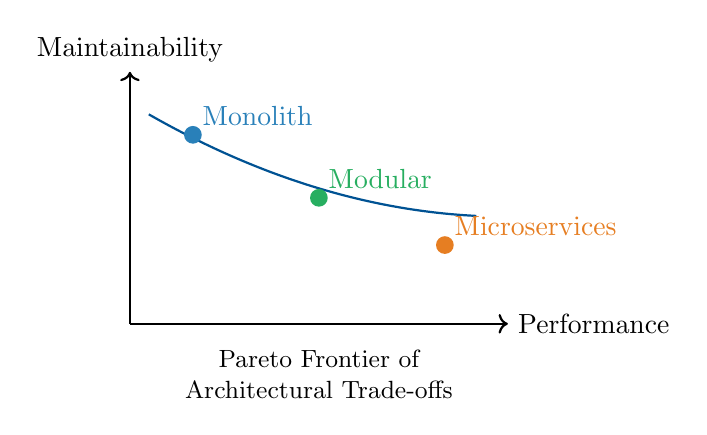
\begin{tikzpicture}[scale=0.8]
    \draw[thick, ->] (0,0) -- (6,0) node[right] {Performance};
    \draw[thick, ->] (0,0) -- (0,4) node[above] {Maintainability};
    
    % Trade-off curve
    \draw[thick, primaryblue, domain=0.3:5.5, smooth] plot (\x, {3.5 - 0.6*\x + 0.05*\x*\x});
    
    % Points
    \fill[trackA] (1,3) circle (4pt) node[above right] {Monolith};
    \fill[accentgreen] (3,2) circle (4pt) node[above right] {Modular};
    \fill[accentorange] (5,1.25) circle (4pt) node[above right] {Microservices};
    
    \node[font=\small, align=center] at (3,-0.8) {Pareto Frontier of\\Architectural Trade-offs};
\end{tikzpicture}
\end{center}

\subsection{Week 3--4: Architecture Styles and Patterns}

\subsubsection{Architecture Styles Covered}

\begin{longtable}{>{\raggedright\arraybackslash}p{3.5cm} >{\raggedright\arraybackslash}p{4cm} >{\raggedright\arraybackslash}p{5cm}}
\toprule
\textbf{Style} & \textbf{Key Characteristics} & \textbf{Best Suited For} \\
\midrule
\endhead
Layered & Separation of concerns, technical partitioning & Traditional enterprise applications \\
\addlinespace
Pipeline & Filters and pipes, data transformation & Data processing, ETL \\
\addlinespace
Microkernel & Core + plugins & IDEs, browsers, extensible systems \\
\addlinespace
Service-Based & Coarse-grained services & Domain-driven decomposition \\
\addlinespace
Event-Driven & Async communication, loose coupling & Real-time systems, IoT \\
\addlinespace
Microservices & Fine-grained, independently deployable & Highly scalable, agile organizations \\
\bottomrule
\end{longtable}

\begin{practicalexercise}
\textbf{Exercise A.1: Architecture Kata}

Design an architecture for an online ordering system with the following requirements:
\begin{itemize}[leftmargin=*]
    \item Support 10,000 concurrent users
    \item 99.9\% availability requirement
    \item Integration with payment providers and inventory systems
    \item Support for mobile and web clients
    \item Real-time order status updates
\end{itemize}
Document your architectural decisions, including:
\begin{enumerate}[leftmargin=*]
    \item The architecture style selected and rationale
    \item Key architectural characteristics prioritized
    \item Component diagram showing major services
    \item Trade-offs accepted and their implications
    \item Fitness functions to validate the architecture
\end{enumerate}
\end{practicalexercise}

\section{Module A.2: Designing Data-Intensive Applications}

\duration{6 weeks} \hfill \bookicon{} \textit{Designing Data-Intensive Applications} by Martin Kleppmann

\begin{bookreference}
\textbf{About This Book:} A highly popular and practical guide for building robust, scalable systems. Kleppmann provides deep insights into the principles behind reliable data systems, covering everything from data models to distributed system challenges.
\end{bookreference}

\subsection{Week 5--6: Foundations of Data Systems}

\subsubsection{Key Concepts}

\textbf{Reliability:} The system continues to work correctly even when things go wrong (hardware faults, software errors, human mistakes).

\textbf{Scalability:} The system can handle growth in data volume, traffic, or complexity through reasonable means.

\textbf{Maintainability:} Different people can work on the system productively over time (operability, simplicity, evolvability).

\subsubsection{Data Models and Query Languages}

Understanding the trade-offs between relational, document, and graph models is essential for making appropriate data store choices.

\begin{center}
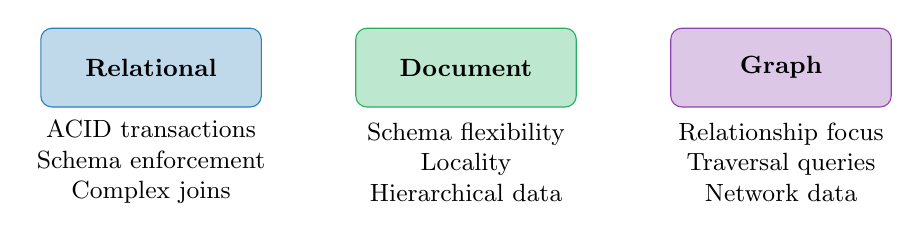
\begin{tikzpicture}[
    model/.style={rectangle, rounded corners, minimum width=2.8cm, minimum height=1cm, text centered, font=\small\bfseries}
]
    \node[model, fill=trackA!30, draw=trackA] (relational) at (0,0) {Relational};
    \node[model, fill=trackB!30, draw=trackB] (document) at (4,0) {Document};
    \node[model, fill=trackC!30, draw=trackC] (graph) at (8,0) {Graph};
    
    \node[font=\small, align=center] at (0,-1.2) {ACID transactions\\Schema enforcement\\Complex joins};
    \node[font=\small, align=center] at (4,-1.2) {Schema flexibility\\Locality\\Hierarchical data};
    \node[font=\small, align=center] at (8,-1.2) {Relationship focus\\Traversal queries\\Network data};
\end{tikzpicture}
\end{center}

\subsection{Week 7--8: Distributed Data}

\subsubsection{Replication Strategies}

Understanding replication is critical for building systems that are both available and consistent. The key replication strategies include:

\textbf{Single-Leader Replication:} One node accepts writes, others replicate. Provides strong consistency but limited write scalability.

\textbf{Multi-Leader Replication:} Multiple nodes accept writes. Better availability but requires conflict resolution.

\textbf{Leaderless Replication:} Any node can accept reads/writes. Maximum availability but requires careful consistency handling.

\subsubsection{Partitioning (Sharding)}

As datasets grow beyond single-node capacity, partitioning becomes essential. Key considerations include:

\begin{itemize}[leftmargin=*]
    \item Partition key selection and its impact on query patterns
    \item Handling hot spots and skewed workloads
    \item Rebalancing strategies as the system grows
    \item Secondary indexes across partitions
\end{itemize}

\subsection{Week 9--10: Consistency and Consensus}

\subsubsection{The CAP Theorem and Beyond}

While the CAP theorem (Consistency, Availability, Partition tolerance---pick two) is foundational, real-world systems operate on a spectrum of consistency models:

\begin{itemize}[leftmargin=*]
    \item \textbf{Linearizability:} Strongest guarantee---operations appear atomic and in real-time order
    \item \textbf{Sequential Consistency:} Operations appear in the same order to all observers
    \item \textbf{Causal Consistency:} Causally related operations are seen in order
    \item \textbf{Eventual Consistency:} Given enough time, all replicas converge
\end{itemize}

\subsubsection{Consensus Algorithms}

Understanding consensus (Paxos, Raft, Zab) is essential for building fault-tolerant distributed systems:

\begin{keyinsight}
Consensus algorithms ensure that all nodes in a distributed system agree on the same values, even in the presence of failures. This is the foundation for leader election, distributed locks, atomic broadcast, and total order delivery.
\end{keyinsight}

\begin{practicalexercise}
\textbf{Exercise A.2: Distributed System Design}

Design a distributed key-value store that meets the following requirements:
\begin{itemize}[leftmargin=*]
    \item Store 100TB of data across 50 nodes
    \item Handle 100,000 reads/second and 10,000 writes/second
    \item Tolerate up to 3 simultaneous node failures
    \item Provide tunable consistency (eventual to strong)
\end{itemize}
Your design should address:
\begin{enumerate}[leftmargin=*]
    \item Partitioning strategy and rebalancing approach
    \item Replication factor and consistency protocol
    \item Failure detection and recovery mechanisms
    \item Client API and consistency level options
\end{enumerate}
\end{practicalexercise}

\section{Module A.3: Distributed Systems Theory}

\duration{4 weeks} \hfill \bookicon{} \textit{Distributed Systems: Principles and Paradigms} by Tanenbaum \& van Steen

\begin{bookreference}
\textbf{About This Book:} A widely recognized textbook covering all key concepts, architectures, and components of distributed systems in depth. It provides the theoretical foundation for understanding how distributed systems work and why they behave as they do.
\end{bookreference}

\subsection{Week 11--12: Communication and Coordination}

\subsubsection{Key Topics}

\begin{itemize}[leftmargin=*]
    \item Remote Procedure Calls (RPC) and message-oriented middleware
    \item Naming and name resolution in distributed systems
    \item Synchronization and logical clocks (Lamport clocks, vector clocks)
    \item Distributed mutual exclusion and election algorithms
\end{itemize}

\subsection{Week 13--14: Fault Tolerance and Security}

\subsubsection{Key Topics}

\begin{itemize}[leftmargin=*]
    \item Failure models and fault classification
    \item Process resilience and group communication
    \item Distributed commit protocols (2PC, 3PC)
    \item Security in distributed systems: authentication, authorization, and secure channels
\end{itemize}

\begin{practicalexercise}
\textbf{Exercise A.3: Failure Mode Analysis}

Take your key-value store design from Exercise A.2 and perform a comprehensive failure mode analysis:
\begin{enumerate}[leftmargin=*]
    \item Identify all possible failure modes (node failures, network partitions, disk failures, etc.)
    \item For each failure mode, document the expected system behavior
    \item Design recovery procedures for each failure type
    \item Create a chaos engineering test plan to validate your fault tolerance
\end{enumerate}
\end{practicalexercise}

\section{Module A.4: Operating System Foundations}

\duration{2 weeks} \hfill \bookicon{} \textit{Operating System Concepts} by Silberschatz, Galvin, \& Gagne

\begin{bookreference}
\textbf{About This Book:} A classic, comprehensive textbook that bridges the gap between operating system concepts and actual implementations. It includes end-of-chapter problems and exercises to reinforce learning.
\end{bookreference}

\subsection{Week 15--16: OS Concepts for Architects}

\subsubsection{Essential Topics for Software Architects}

While not every software architect needs to understand OS internals deeply, certain concepts directly impact application design:

\begin{itemize}[leftmargin=*]
    \item \textbf{Process and Thread Management:} Understanding scheduling, context switching, and concurrency primitives
    \item \textbf{Memory Management:} Virtual memory, paging, and their impact on application performance
    \item \textbf{I/O and File Systems:} Understanding how I/O operations work at the OS level
    \item \textbf{Virtualization and Containers:} How modern deployment targets differ from bare metal
\end{itemize}

\begin{keyinsight}
Understanding OS-level concepts helps architects make better decisions about concurrency models, memory usage patterns, and deployment strategies. The abstractions provided by programming languages and frameworks rest on these OS primitives.
\end{keyinsight}

% ============================================================================
% CHAPTER 4: TRACK B - SYSTEMS ENGINEERING
% ============================================================================
\chapter{Track B: Systems Engineering}

\begin{trackbox}[\ding{72} Track B: Systems Engineering]{trackB}
This track develops expertise in the disciplined approach to designing, developing, and managing complex systems throughout their lifecycle. It covers both theoretical principles and practical application of systems engineering methodologies.
\end{trackbox}

\vspace{0.5cm}
\duration{8 weeks} \hfill \difficulty{Intermediate}

\begin{prerequisitebox}
\begin{itemize}[leftmargin=*]
    \item Completion of Phase 1: Foundational Systems Thinking
    \item Understanding of project management fundamentals
    \item Experience working on multi-disciplinary projects
\end{itemize}
\end{prerequisitebox}

\begin{learningobjectives}
\begin{itemize}[leftmargin=*]
    \item Understand the systems engineering lifecycle and key processes
    \item Apply requirements engineering techniques effectively
    \item Design systems using structured decomposition methods
    \item Manage system integration and verification
    \item Balance technical and programmatic concerns in system development
\end{itemize}
\end{learningobjectives}

\section{Module B.1: Systems Engineering Principles}

\duration{5 weeks} \hfill \bookicon{} \textit{Systems Engineering Principles and Practice} by Alexander Kossiakoff

\begin{bookreference}
\textbf{About This Book:} A comprehensive textbook used in professional and academic settings to understand the core principles and practical application of systems engineering. It covers the full lifecycle from concept development through operations and retirement.
\end{bookreference}

\subsection{Week 1--2: The Systems Engineering Process}

\subsubsection{The Vee Model}

The Vee Model provides a framework for understanding the systems engineering lifecycle:

\begin{center}
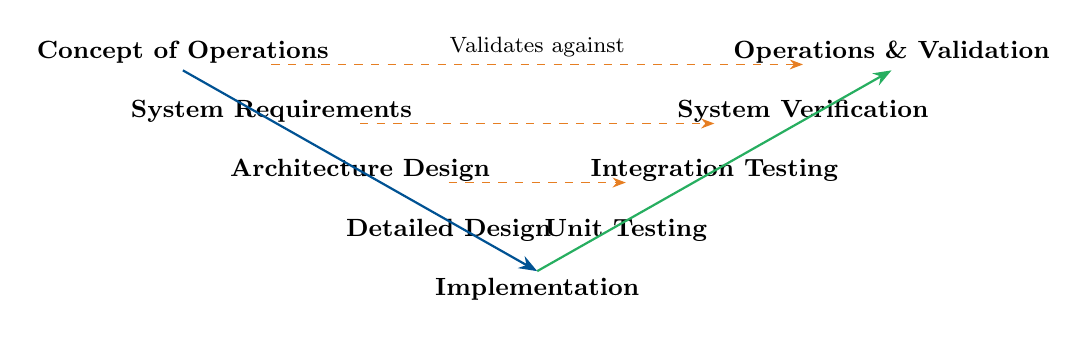
\begin{tikzpicture}[scale=0.75]
    % Left side (decomposition)
    \node[font=\small\bfseries] at (0,4.5) {Concept of Operations};
    \node[font=\small\bfseries] at (1.5,3.5) {System Requirements};
    \node[font=\small\bfseries] at (3,2.5) {Architecture Design};
    \node[font=\small\bfseries] at (4.5,1.5) {Detailed Design};
    \node[font=\small\bfseries] at (6,0.5) {Implementation};
    
    % Right side (integration)
    \node[font=\small\bfseries] at (12,4.5) {Operations \& Validation};
    \node[font=\small\bfseries] at (10.5,3.5) {System Verification};
    \node[font=\small\bfseries] at (9,2.5) {Integration Testing};
    \node[font=\small\bfseries] at (7.5,1.5) {Unit Testing};
    
    % Vee shape
    \draw[thick, primaryblue, -{Stealth}] (0,4.2) -- (6,0.8);
    \draw[thick, accentgreen, -{Stealth}] (6,0.8) -- (12,4.2);
    
    % Horizontal arrows
    \draw[dashed, accentorange, -{Stealth}] (1.5,4.3) -- (10.5,4.3);
    \draw[dashed, accentorange, -{Stealth}] (3,3.3) -- (9,3.3);
    \draw[dashed, accentorange, -{Stealth}] (4.5,2.3) -- (7.5,2.3);
    
    \node[font=\footnotesize] at (6,4.6) {Validates against};
\end{tikzpicture}
\end{center}

\subsubsection{Key Processes}

\begin{itemize}[leftmargin=*]
    \item \textbf{Requirements Engineering:} Eliciting, analyzing, specifying, and validating requirements
    \item \textbf{Functional Analysis:} Decomposing system functions into manageable elements
    \item \textbf{Design Synthesis:} Creating physical solutions that satisfy functional requirements
    \item \textbf{Verification and Validation:} Ensuring the system meets requirements and user needs
\end{itemize}

\subsection{Week 3--4: Requirements and Architecture}

\subsubsection{Requirements Hierarchy}

\begin{center}
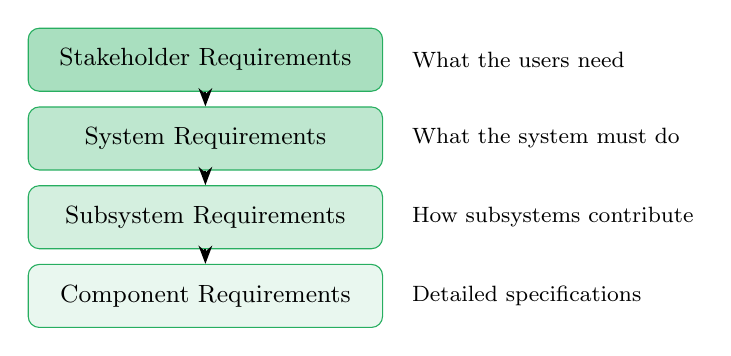
\begin{tikzpicture}[
    level/.style={rectangle, rounded corners, minimum width=4.5cm, minimum height=0.8cm, text centered, font=\small},
    level 1/.style={level, fill=trackB!40, draw=trackB},
    level 2/.style={level, fill=trackB!30, draw=trackB},
    level 3/.style={level, fill=trackB!20, draw=trackB},
    level 4/.style={level, fill=trackB!10, draw=trackB}
]
    \node[level 1] (stakeholder) at (0,3) {Stakeholder Requirements};
    \node[level 2] (system) at (0,2) {System Requirements};
    \node[level 3] (subsystem) at (0,1) {Subsystem Requirements};
    \node[level 4] (component) at (0,0) {Component Requirements};
    
    \draw[thick, -{Stealth}] (stakeholder) -- (system);
    \draw[thick, -{Stealth}] (system) -- (subsystem);
    \draw[thick, -{Stealth}] (subsystem) -- (component);
    
    \node[font=\footnotesize, right] at (2.5,3) {What the users need};
    \node[font=\footnotesize, right] at (2.5,2) {What the system must do};
    \node[font=\footnotesize, right] at (2.5,1) {How subsystems contribute};
    \node[font=\footnotesize, right] at (2.5,0) {Detailed specifications};
\end{tikzpicture}
\end{center}

\subsection{Week 5: Integration and Life Cycle Management}

\subsubsection{Key Topics}

\begin{itemize}[leftmargin=*]
    \item System integration strategies (big bang vs. incremental)
    \item Test planning and execution
    \item Configuration management
    \item Operations, maintenance, and system retirement
\end{itemize}

\begin{practicalexercise}
\textbf{Exercise B.1: Requirements Decomposition}

For the ordering system architecture you designed in Exercise A.1, create a formal requirements specification:
\begin{enumerate}[leftmargin=*]
    \item Write 5 stakeholder requirements (user perspective)
    \item Derive 15 system requirements from the stakeholder requirements
    \item Create traceability matrix linking stakeholder to system requirements
    \item Define verification methods for each system requirement
    \item Identify potential requirement conflicts and propose resolutions
\end{enumerate}
\end{practicalexercise}

\section{Module B.2: Practical Systems Engineering}

\duration{3 weeks} \hfill \bookicon{} \textit{The Art of Systems Engineering} by Marco Chicherio

\begin{bookreference}
\textbf{About This Book:} A practical guide focusing on the problem-solving and design aspects of systems engineering. This book emphasizes the craft and judgment required in real-world SE practice.
\end{bookreference}

\subsection{Week 6--8: Applied Systems Engineering}

\subsubsection{Key Focus Areas}

\begin{itemize}[leftmargin=*]
    \item Problem structuring and stakeholder analysis
    \item Trade study methodologies and decision-making frameworks
    \item Interface management and integration planning
    \item Risk identification and mitigation strategies
    \item Technical reviews and decision gates
\end{itemize}

\begin{practicalexercise}
\textbf{Exercise B.2: Trade Study}

Conduct a formal trade study for the data storage layer of your ordering system:
\begin{enumerate}[leftmargin=*]
    \item Define evaluation criteria and weighting factors
    \item Identify at least 3 alternative solutions
    \item Score each alternative against the criteria
    \item Document assumptions and sensitivity analysis
    \item Present recommendations with supporting rationale
\end{enumerate}
\end{practicalexercise}

% ============================================================================
% CHAPTER 5: TRACK C - SOFTWARE DEVELOPMENT
% ============================================================================
\chapter{Track C: Software Development Practice}

\begin{trackbox}[\ding{72} Track C: Software Development]{trackC}
This track develops expertise in the craft of software development, covering object-oriented design principles, project management challenges, and modern engineering practices. It bridges the gap between architecture and implementation.
\end{trackbox}

\vspace{0.5cm}
\duration{10 weeks} \hfill \difficulty{Beginner to Intermediate}

\begin{prerequisitebox}
\begin{itemize}[leftmargin=*]
    \item Completion of Phase 1: Foundational Systems Thinking
    \item Programming experience in an object-oriented language
    \item Basic understanding of software development workflows
\end{itemize}
\end{prerequisitebox}

\begin{learningobjectives}
\begin{itemize}[leftmargin=*]
    \item Apply object-oriented design principles to create flexible, maintainable code
    \item Understand the human and organizational aspects of software projects
    \item Apply modern software engineering practices effectively
    \item Navigate the trade-offs between design purity and practical constraints
    \item Lead and contribute to software projects more effectively
\end{itemize}
\end{learningobjectives}

\section{Module C.1: Object-Oriented Design}

\duration{4 weeks} \hfill \bookicon{} \textit{Practical Object-Oriented Design} by Sandi Metz

\begin{bookreference}
\textbf{About This Book:} A highly relevant and practical book offering object-oriented design techniques that lead to code that is easy to understand, change, and extend. Metz focuses on managing dependencies and creating flexible designs.
\end{bookreference}

\subsection{Week 1--2: Designing Classes with Purpose}

\subsubsection{Single Responsibility and Managing Dependencies}

\textbf{Single Responsibility Principle:} A class should have only one reason to change. This doesn't mean a class should do only one thing, but rather that everything it does should be highly related.

\textbf{Dependency Management:} The direction and nature of dependencies determines how easily code can change:

\begin{itemize}[leftmargin=*]
    \item Depend on things that change less frequently than you do
    \item Depend on abstractions, not concretions
    \item Inject dependencies rather than hard-coding them
\end{itemize}

\begin{keyinsight}
Design is the art of arranging code to minimize the cost of change. Good design doesn't cost more---it costs less over the lifetime of the software because it reduces the effort required to add features and fix bugs.
\end{keyinsight}

\subsection{Week 3--4: Flexible Interfaces and Inheritance}

\subsubsection{Key Concepts}

\textbf{Duck Typing:} Focus on what objects do, not what they are. If it walks like a duck and quacks like a duck, treat it like a duck.

\textbf{Composition over Inheritance:} Prefer object composition to class inheritance. Inheritance creates tight coupling, while composition allows more flexible relationships.

\textbf{Interface Design:} Good interfaces are minimal, complete, and stable. They define what messages an object responds to without exposing implementation details.

\begin{practicalexercise}
\textbf{Exercise C.1: Refactoring for Flexibility}

Take an existing codebase (your own or an open-source project) and:
\begin{enumerate}[leftmargin=*]
    \item Identify a class with multiple responsibilities
    \item Refactor it into multiple single-responsibility classes
    \item Identify hard-coded dependencies and inject them
    \item Create interfaces/protocols for the dependencies
    \item Write tests that use test doubles for the dependencies
\end{enumerate}
Document how these changes affect testability and changeability.
\end{practicalexercise}

\section{Module C.2: The Human Side of Software}

\duration{3 weeks} \hfill \bookicon{} \textit{The Mythical Man-Month} by Frederick Brooks Jr.

\begin{bookreference}
\textbf{About This Book:} A classic in software engineering that discusses project management fundamentals, including the famous Brooks's Law: ``Adding manpower to a late software project makes it later.'' Despite being decades old, its insights remain remarkably relevant.
\end{bookreference}

\subsection{Week 5--6: Essential Concepts}

\subsubsection{Brooks's Law and Its Implications}

\begin{center}
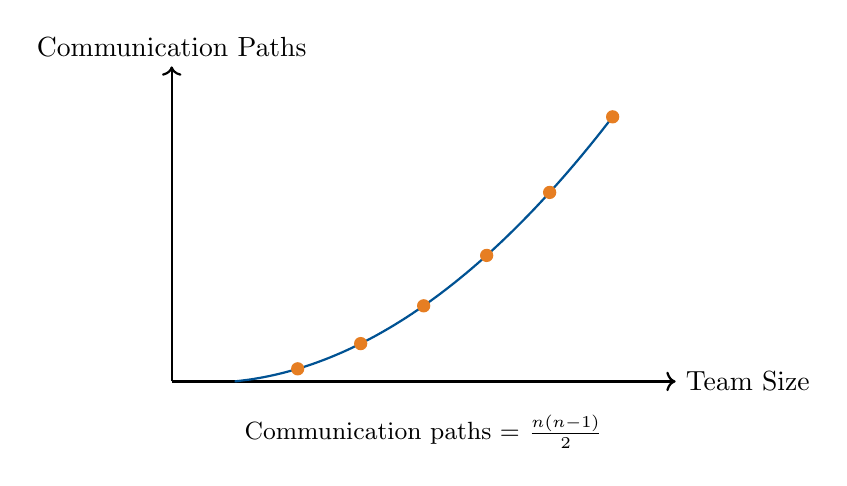
\begin{tikzpicture}[scale=0.8]
    \draw[thick, ->] (0,0) -- (8,0) node[right] {Team Size};
    \draw[thick, ->] (0,0) -- (0,5) node[above] {Communication Paths};
    
    % n(n-1)/2 curve
    \draw[thick, primaryblue, domain=1:7, smooth] plot (\x, {0.1*\x*(\x-1)});
    
    % Points
    \foreach \n in {2,3,4,5,6,7} {
        \pgfmathsetmacro{\y}{0.1*\n*(\n-1)}
        \fill[accentorange] (\n,\y) circle (3pt);
    }
    
    \node[font=\small] at (4,-0.8) {Communication paths = $\frac{n(n-1)}{2}$};
\end{tikzpicture}
\end{center}

\subsubsection{The Surgical Team Model}

Brooks proposed organizing teams around a ``chief programmer'' (like a surgical team around a surgeon), with specialized supporting roles:

\begin{itemize}[leftmargin=*]
    \item Chief Programmer: The surgeon who does the core work
    \item Copilot: A peer who can step in and provides second opinion
    \item Administrator: Handles money, people, space, machines
    \item Editor: Maintains documentation
    \item Toolsmith: Builds specialized tools for the chief
\end{itemize}

\subsection{Week 7: The Second-System Effect and Other Insights}

\subsubsection{Key Concepts}

\textbf{Second-System Effect:} The second system a designer builds is often over-engineered, as they try to include all the features they wished they had in the first.

\textbf{Plan to Throw One Away:} The first version of a system will be a learning experience. Plan for it.

\textbf{Conceptual Integrity:} A system should have a coherent vision. One mind (or a small group with shared vision) should be responsible for design.

\begin{practicalexercise}
\textbf{Exercise C.2: Project Retrospective Analysis}

Reflect on a project you've participated in:
\begin{enumerate}[leftmargin=*]
    \item Identify instances where Brooks's Law applied
    \item Analyze how communication overhead affected productivity
    \item Evaluate whether conceptual integrity was maintained
    \item Identify second-system effect symptoms if present
    \item Propose changes based on Brooks's insights
\end{enumerate}
\end{practicalexercise}

\section{Module C.3: Modern Software Engineering}

\duration{3 weeks} \hfill \bookicon{} \textit{Modern Software Engineering} by David Farley

\begin{bookreference}
\textbf{About This Book:} A recent take on building better software faster, focusing on practical principles and practices. Farley emphasizes empirical approaches, fast feedback, and continuous improvement as foundations for effective software development.
\end{bookreference}

\subsection{Week 8--10: Engineering Excellence}

\subsubsection{Core Principles}

\textbf{Working Iteratively:} Break work into small, valuable increments that can be completed and validated quickly.

\textbf{Fast Feedback:} Reduce the time between making a change and learning about its effects. This applies to testing, deployment, and user feedback.

\textbf{Working Incrementally:} Build systems in small steps, each of which adds value and can be validated independently.

\textbf{Experimentation:} Treat development as a series of experiments. Form hypotheses, test them, and learn from the results.

\subsubsection{Modern Practices}

\begin{itemize}[leftmargin=*]
    \item Continuous Integration and Continuous Delivery (CI/CD)
    \item Test-Driven Development (TDD) and Behavior-Driven Development (BDD)
    \item Trunk-based development and feature flags
    \item Infrastructure as Code and GitOps
    \item Observability and monitoring
\end{itemize}

\begin{practicalexercise}
\textbf{Exercise C.3: CI/CD Pipeline Design}

Design a complete CI/CD pipeline for the ordering system:
\begin{enumerate}[leftmargin=*]
    \item Define the stages from commit to production
    \item Specify the automated tests at each stage
    \item Design the deployment strategy (blue-green, canary, etc.)
    \item Include observability and rollback mechanisms
    \item Document how the pipeline enables fast feedback
\end{enumerate}
\end{practicalexercise}

% ============================================================================
% CHAPTER 6: TRACK D - BUSINESS SYSTEMS
% ============================================================================
\chapter{Track D: Business Systems and Process Design}

\begin{trackbox}[\ding{72} Track D: Business Systems]{trackD}
This track develops expertise in building, documenting, and optimizing business processes and organizational systems. It provides the non-technical foundations that enable technical systems to create value within organizations.
\end{trackbox}

\vspace{0.5cm}
\duration{10 weeks} \hfill \difficulty{Beginner to Intermediate}

\begin{prerequisitebox}
\begin{itemize}[leftmargin=*]
    \item Completion of Phase 1: Foundational Systems Thinking
    \item Basic understanding of business operations
    \item Interest in organizational design and process improvement
\end{itemize}
\end{prerequisitebox}

\begin{learningobjectives}
\begin{itemize}[leftmargin=*]
    \item Understand why systems are crucial for business success
    \item Document and optimize business processes effectively
    \item Create organizational structures that enable scaling
    \item Apply service design methodologies to process improvement
    \item Integrate technical and business systems thinking
\end{itemize}
\end{learningobjectives}

\section{Module D.1: The Importance of Business Systems}

\duration{2 weeks} \hfill \bookicon{} \textit{The E-Myth Revisited} by Michael Gerber

\begin{bookreference}
\textbf{About This Book:} Excellent for understanding the importance of systems in small businesses, serving as a foundation before diving into specifics. Gerber explains why most small businesses fail and how systematization is the key to success.
\end{bookreference}

\subsection{Week 1--2: Working ON vs. IN the Business}

\subsubsection{The Three Roles}

Gerber identifies three personas within every business owner:

\begin{itemize}[leftmargin=*]
    \item \textbf{The Technician:} Wants to do the work; lives in the present
    \item \textbf{The Manager:} Wants to organize and plan; lives in the past
    \item \textbf{The Entrepreneur:} Wants to create and innovate; lives in the future
\end{itemize}

\subsubsection{The Franchise Prototype}

The key insight is treating your business as if it were the prototype for a franchise:

\begin{keyinsight}
A business that depends on you (the owner) for its operation is not a business---it's a job. The goal is to create systems that allow the business to run without your direct involvement, producing consistent results regardless of who executes them.
\end{keyinsight}

\section{Module D.2: Process Documentation}

\duration{3 weeks} \hfill \bookicon{} \textit{Work the System} by Sam Carpenter

\begin{bookreference}
\textbf{About This Book:} Offers practical, actionable steps for documenting and improving business processes. Carpenter provides a methodology for identifying, documenting, and optimizing the systems that run your business.
\end{bookreference}

\subsection{Week 3--5: Systems Documentation Method}

\subsubsection{The Three Documents}

Carpenter's methodology centers on three core documents:

\begin{enumerate}[leftmargin=*]
    \item \textbf{Strategic Objective:} A one- to two-page description of what you want your business to be
    \item \textbf{Operating Principles:} The guiding principles for decision-making
    \item \textbf{Working Procedures:} Detailed documentation of how each task is performed
\end{enumerate}

\subsubsection{Creating Working Procedures}

Effective working procedures should be:

\begin{itemize}[leftmargin=*]
    \item Written by the person who does the work
    \item Specific enough that anyone could follow them
    \item Updated whenever the process changes
    \item Reviewed regularly for improvement opportunities
\end{itemize}

\begin{practicalexercise}
\textbf{Exercise D.1: Process Documentation}

Select a key process in your work (e.g., code review, incident response, deployment):
\begin{enumerate}[leftmargin=*]
    \item Document the current process step-by-step
    \item Identify decision points and their criteria
    \item Note where the process breaks down or varies
    \item Create a standardized procedure document
    \item Identify metrics to measure process effectiveness
\end{enumerate}
\end{practicalexercise}

\section{Module D.3: Organizational Systems}

\duration{2 weeks} \hfill \bookicon{} \textit{Traction} by Gino Wickman

\begin{bookreference}
\textbf{About This Book:} Provides tools to create a vision and develop an organizational structure, which are essential for building any system. The Entrepreneurial Operating System (EOS) offers a comprehensive framework for running a business.
\end{bookreference}

\subsection{Week 6--7: The EOS Framework}

\subsubsection{Six Key Components}

The Entrepreneurial Operating System addresses six components:

\begin{enumerate}[leftmargin=*]
    \item \textbf{Vision:} Getting everyone aligned on where you're going and how you'll get there
    \item \textbf{People:} Having the right people in the right seats
    \item \textbf{Data:} Running your business on objective information
    \item \textbf{Issues:} Identifying and solving problems systematically
    \item \textbf{Process:} Documenting and following core processes
    \item \textbf{Traction:} Bringing discipline and accountability to the organization
\end{enumerate}

\section{Module D.4: Scaling Systems}

\duration{1 week} \hfill \bookicon{} \textit{Scaling Up} by Verne Harnish

\begin{bookreference}
\textbf{About This Book:} Focuses on how to scale a business, which involves building and refining systems to handle growth. Harnish provides practical tools for managing the four key areas: People, Strategy, Execution, and Cash.
\end{bookreference}

\subsection{Week 8: Growth Systems}

\subsubsection{The Four Decisions}

Scaling a business requires mastering four key areas:

\begin{itemize}[leftmargin=*]
    \item \textbf{People:} Attracting, developing, and retaining the right team
    \item \textbf{Strategy:} Differentiating and aligning the organization
    \item \textbf{Execution:} Driving accountability and alignment
    \item \textbf{Cash:} Generating enough cash to fuel growth
\end{itemize}

\section{Module D.5: Service Design}

\duration{2 weeks} \hfill \bookicon{} \textit{Service Design Doing}

\begin{bookreference}
\textbf{About This Book:} A technical and comprehensive textbook on designing and optimizing any process, from point A to point B. It uses diagrams to visualize flow and provides tools for creating exceptional service experiences.
\end{bookreference}

\subsection{Week 9--10: Design Thinking for Processes}

\subsubsection{Key Methodologies}

\begin{itemize}[leftmargin=*]
    \item \textbf{Journey Mapping:} Visualizing the end-to-end experience
    \item \textbf{Service Blueprinting:} Documenting frontstage and backstage activities
    \item \textbf{Stakeholder Mapping:} Understanding all parties involved
    \item \textbf{Prototyping Services:} Testing service designs before implementation
\end{itemize}

\begin{practicalexercise}
\textbf{Exercise D.2: Service Blueprint}

Create a service blueprint for the ordering process in your system:
\begin{enumerate}[leftmargin=*]
    \item Map the customer journey from discovery to delivery
    \item Document the frontstage interactions (what customer sees)
    \item Document the backstage processes (what happens behind the scenes)
    \item Identify support processes and systems
    \item Mark pain points and opportunities for improvement
\end{enumerate}
\end{practicalexercise}

% ============================================================================
% CHAPTER 7: CAPSTONE INTEGRATION
% ============================================================================
\chapter{Phase 5: Capstone Integration and Application}

\duration{12 weeks} \hfill \difficulty{Advanced}

This final phase integrates learning from all tracks into a comprehensive capstone project. Participants synthesize their knowledge by designing, documenting, and potentially implementing a complete system that demonstrates mastery across all domains.

\begin{learningobjectives}
\begin{itemize}[leftmargin=*]
    \item Integrate systems thinking with technical architecture
    \item Apply software engineering best practices in a realistic context
    \item Create comprehensive documentation spanning all aspects of a system
    \item Demonstrate ability to make and justify architectural trade-offs
    \item Present complex technical concepts to diverse stakeholders
\end{itemize}
\end{learningobjectives}

\section{Capstone Project: Complete Ordering System}

\subsection{Project Scope}

Design and document a complete ordering system that incorporates:

\begin{enumerate}[leftmargin=*]
    \item \textbf{Systems Thinking Analysis:} Causal loop diagrams, leverage point identification, and resilience analysis
    \item \textbf{Software Architecture:} Complete architectural documentation including ADRs, component diagrams, and deployment architecture
    \item \textbf{Distributed Systems Design:} Data partitioning strategy, consistency model, and fault tolerance approach
    \item \textbf{Systems Engineering Artifacts:} Requirements specification, traceability matrix, and verification plan
    \item \textbf{Software Development Plan:} Object model, coding standards, and CI/CD pipeline design
    \item \textbf{Business Systems:} Process documentation, organizational structure, and service blueprint
\end{enumerate}

\subsection{Deliverables}

\subsubsection{Phase 1: Analysis (Weeks 1--3)}
\begin{itemize}[leftmargin=*]
    \item Stakeholder analysis and requirements elicitation
    \item System context diagram and boundary definition
    \item Causal loop diagram of the complete system
    \item Initial architectural hypothesis
\end{itemize}

\subsubsection{Phase 2: Design (Weeks 4--7)}
\begin{itemize}[leftmargin=*]
    \item Complete software architecture documentation
    \item Data model and partitioning strategy
    \item Interface specifications
    \item Integration architecture
\end{itemize}

\subsubsection{Phase 3: Implementation Planning (Weeks 8--10)}
\begin{itemize}[leftmargin=*]
    \item Development team structure and responsibilities
    \item CI/CD pipeline specification
    \item Testing strategy
    \item Operations runbook
\end{itemize}

\subsubsection{Phase 4: Presentation (Weeks 11--12)}
\begin{itemize}[leftmargin=*]
    \item Executive summary for business stakeholders
    \item Technical deep-dive for engineering teams
    \item Risk assessment and mitigation plan
    \item Lessons learned and recommendations
\end{itemize}

\section{Assessment Criteria}

\begin{longtable}{>{\raggedright\arraybackslash}p{4cm} >{\raggedright\arraybackslash}p{2cm} >{\raggedright\arraybackslash}p{7.5cm}}
\toprule
\textbf{Criterion} & \textbf{Weight} & \textbf{Description} \\
\midrule
\endhead
Systems Thinking Application & 15\% & Effective use of systems thinking concepts throughout \\
\addlinespace
Architectural Quality & 20\% & Appropriate architecture style, clear trade-offs, fitness functions \\
\addlinespace
Technical Depth & 20\% & Thorough treatment of distributed systems, data design \\
\addlinespace
Documentation Quality & 15\% & Clear, complete, maintainable documentation \\
\addlinespace
Process Integration & 15\% & Effective integration of business and technical processes \\
\addlinespace
Presentation Quality & 15\% & Clear communication to varied audiences \\
\bottomrule
\end{longtable}

% ============================================================================
% CHAPTER 8: APPENDICES
% ============================================================================
\appendix

\chapter{Complete Reading Schedule}

\section{52-Week Master Schedule}

\begin{longtable}{>{\raggedright\arraybackslash}p{1.5cm} >{\raggedright\arraybackslash}p{4cm} >{\raggedright\arraybackslash}p{5cm} >{\raggedright\arraybackslash}p{3cm}}
\toprule
\textbf{Week} & \textbf{Phase/Track} & \textbf{Book/Focus} & \textbf{Hours/Week} \\
\midrule
\endhead
1--4 & Foundation & Thinking in Systems & 10--12 \\
5--8 & Foundation & General Systems Thinking & 10--12 \\
\midrule
9--12 & Track A & Fundamentals of Software Architecture & 12--15 \\
13--18 & Track A & Designing Data-Intensive Applications & 12--15 \\
19--22 & Track A & Distributed Systems (selected chapters) & 12--15 \\
23--24 & Track A & Operating System Concepts (selected) & 10--12 \\
\midrule
25--29 & Track B & Systems Engineering Principles & 10--12 \\
30--32 & Track B & The Art of Systems Engineering & 10--12 \\
\midrule
33--36 & Track C & Practical Object-Oriented Design & 12--15 \\
37--39 & Track C & The Mythical Man-Month & 8--10 \\
40--42 & Track C & Modern Software Engineering & 10--12 \\
\midrule
43--44 & Track D & The E-Myth Revisited & 8--10 \\
45--47 & Track D & Work the System & 10--12 \\
48 & Track D & Traction (core chapters) & 8--10 \\
49 & Track D & Scaling Up (selected chapters) & 8--10 \\
50 & Track D & Service Design Doing (selected) & 10--12 \\
\midrule
51--52 & Capstone & Integration Project & 15--20 \\
\bottomrule
\end{longtable}

\chapter{Supplementary Resources}

\section{Online Resources}

\begin{itemize}[leftmargin=*]
    \item Martin Fowler's Architecture Guide: \url{https://martinfowler.com/architecture/}
    \item The Systems Thinker: \url{https://thesystemsthinker.com/}
    \item InfoQ Software Architecture: \url{https://www.infoq.com/software-architecture/}
    \item INCOSE Systems Engineering Handbook (reference)
\end{itemize}

\section{Related Academic Courses}

\begin{itemize}[leftmargin=*]
    \item MIT OpenCourseWare: Introduction to Systems Engineering
    \item Stanford Online: Distributed Systems
    \item Carnegie Mellon Software Engineering Institute resources
\end{itemize}

\chapter{Glossary of Key Terms}

\begin{description}[leftmargin=2cm, labelwidth=1.8cm]
    \item[ADR] Architecture Decision Record---document capturing important architectural decisions
    \item[CAP] Consistency, Availability, Partition tolerance theorem
    \item[CI/CD] Continuous Integration/Continuous Delivery
    \item[DDIA] Designing Data-Intensive Applications (Kleppmann)
    \item[EOS] Entrepreneurial Operating System (Wickman)
    \item[OO] Object-Oriented (design/programming)
    \item[SE] Systems Engineering
    \item[SRP] Single Responsibility Principle
    \item[TDD] Test-Driven Development
\end{description}

% ============================================================================
% END MATTER
% ============================================================================
\vfill
\begin{center}
\rule{0.6\textwidth}{0.4pt}\\[0.5cm]
{\Large\bfseries\color{primaryblue} End of Curriculum}\\[0.3cm]
{\small Version 1.0 --- Comprehensive Systems Engineering and Software Architecture Program}
\end{center}

\end{document}